\chapter{Fortran Programs}

%%%%%%%
%  Section
%%%%%%%
\section{Example Programs}

To do parallel programming using OpenMP or MPI (Message passing interface), we typically need to use a lower level language than Matlab such as Fortran. Another possible choice of language is C, however Fortran has superior array handling capabilities compared to C, and has a similar syntax to Matlab, so is typically easier to use for scientific computations which make heavy use of regular arrays. It is therefore useful to introduce a few simple programs in Fortran before we begin studying how to create parallel programs. A good recent reference on Fortran is Metcalf, Reid and Cohen~\cite{MetReiCoh11}.  We recognize that most people will be unfamiliar with Fortran and probably more familiar with Matlab\footnote{Although Matlab is written in C, it was originally written in Fortran and so has a similar style to Fortran.}, C or C++, but we expect that the example codes will make it easy for anyone with some introductory programming background.   A recent guide which describes how to write efficient parallel Fortran code is Levesque and Wagenbreth\cite{LevWag11}. Our programs are written to be run on the Flux cluster at the University of Michigan. More information on this cluster can be found at \url{http://cac.engin.umich.edu/resources/systems/flux/} and at \url{http://cac.engin.umich.edu/started/index.html}. Below are four files you will need to run this.

\begin{enumerate}
\item[1)] A makefile to compile the Fortran code on Flux in listing \ref{lst:MakefileHeat}. This should be saved as {\it makefile}. Before using the makefile to compile the code, you will need to type\\
\texttt{module load fftw/3.2.1-intel}\\
at the command line prompt once logged into Flux. Then place the makefile and heat.f90 in the same directory, the example files below assume this directory is\\
\texttt{\${HOME}/ParallelMethods/Heat}\\
 and type\\
\texttt{make}\\
to compile the file. Once the file is compiled type\\
\texttt{qsub fluxsubscript}\\
to get the cluster to run your program and then output the results. The programs that follow use the library FFTW to do the fast Fourier Transforms. More information on this library can be found at \url{http://www.fftw.org/}.

\lstinputlisting[style=make_style,language=make,label=lst:MakefileHeat,caption={An example makefile for compiling a Fourier spectral Fortran heat equation program.}]{./FortranPrograms/Programs/FortranHeatEquation/makefile}

\item[2)] The Fortran program in listing \ref{lst:FortranHeat} -- this should be saved as {\it heat.f90}
\lstinputlisting[style=fortran_style,language=Fortran,label=lst:FortranHeat,caption={A Fortran Fourier spectral program to solve the heat equation using backward Euler timestepping.}]{./FortranPrograms/Programs/FortranHeatEquation/heat.f90}

\item[3]) An example submission script to use on the cluster in Listing \ref{lst:Fluxsubheat} -- this should be saved as {\it fluxsubscript}. More examples can be found at \url{http://cac.engin.umich.edu/resources/software/pbs.html}. To use it, please change the email address from \url{your_uniqname@umich.edu} to an email address at which you can receive notifications of when jobs start and are finished. 

\lstinputlisting[style=bash_style,language=bash,label=lst:Fluxsubheat,caption={An example submission script for use on Flux.}]{./FortranPrograms/Programs/FortranHeatEquation/fluxsubscript}

\item[4)] A Matlab plotting script\footnote{For many computational problems, one can visualize the results with 10-100 times less computational power than was needed to generate the results, so for problems which are not too large, it is much easier to use a high level language like Matlab to post-process the data.} to generate Fig.\ \ref{fig:FortranHeat} is in listing \ref{lst:PlotMatlab}.

\lstinputlisting[style=matlab_style,label=lst:PlotMatlab,caption={A Matlab program to plot the computed results.}]{./FortranPrograms/Programs/FortranHeatEquation/plotcreate.m}

\begin{figure}
\begin{center}
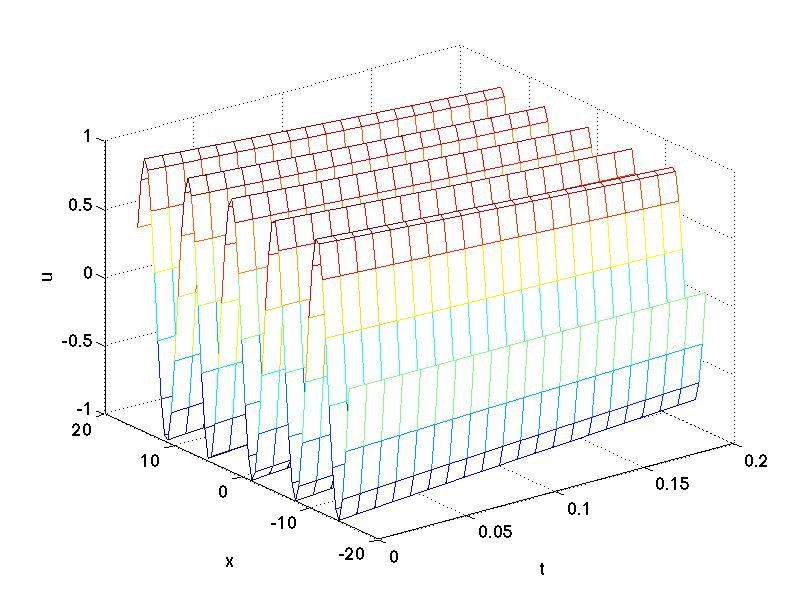
\includegraphics[scale=.35]{./FortranPrograms/heatPlot.jpg}
\caption{The solution to the heat equation computed by Fortran and post-processed by Matlab.} \label{fig:FortranHeat}
\end{center}
\end{figure}

\end{enumerate}


%%%%%%%
%  Section
%%%%%%%
\section{Exercises}
\begin{enumerate}
\item[1)] Please read the resources on the web page \url{http://cac.engin.umich.edu/started/index.html} to learn how to use the Flux cluster.
\item[2)] Modify the Fortran program for the 1-D heat equation to solve the Allen-Cahn equation, with your choice of time stepping scheme. Create a plot of the output of your run. Include the source code and plot in your solutions.
\item[3)] Modify the Fortran program for the 1-D heat equation to solve the  2-D heat equation with your choice of time stepping scheme. Your program should save the field at each time step rather than putting all the fields in a single large array. Create a plot of the initial and final states of your run. Include the source code and plots in your solutions.
\end{enumerate}

